\chapter*{Web-Visualisierung}\thispagestyle{fancy}\markboth{Web-Visualisierung}{}
\addcontentsline{toc}{chapter}{Web-Visualisierung}

\section{Besprechung mit Kollegen �ber Inhalt/Design}

\large
{Ab November soll ein neues Projekt entstehen, welches das Ziel hat, einige gemessene und gesendete Daten einer Kraftwerk, mittels eine Website  visualisieren. Am Anfang war das Projekt-Zielstellung besprochen worden. In diese Besprechungen wurden die jeweiligen Aufgaben verteilt. Die Abteilung Eingebete Systeme soll einen Apache Server mit PHP installieren und eine postgreSQL Datenbank, wo alle Werten aus eine Kraftwerk gespeichert werden, erstellen. Mir war die Visualisierung von diese Daten zugeordnet. Die visualisierte Daten sollen in einer Website dargestellt werden. \\
Die Daten aus einer Kraftwerk sollen �bersichtlich und mittels Diagrammen visualisiert werden. Es war festgelegt, welche Daten zu visualisieren geeignet sind. Es war auch besprochen, welche Mitteln f�r die Website Erstellung geeignet sind. Dazu geh�ren Bootstrap Frameworks, jQuery und dazugeh�rige Software f�r die Bearbeitung.}

% erstmals einen Projekt Plan erstellt, Besprechung\\

% jeweiligen aufgaben verteilen = Eingebete Systeme sollen eine Apache Server mit PHP, ich soll die Website, Design und Konzept entwickeln\\

% definieren was wird visualisiert, Was ist unsere ziel? (genauer definieren) = Daten eine Kraftwerk �bersichtlich darstellen und im Diagrammen anzeigen\\




\section{Konzept f�r die Oberfl�che mittels Skizzen und grafischer Software}

\Large{Es soll ein Konzept f�r die Website entwickelt werden. Es wird ein Konzept mit grafisches Programm GIMP gemacht, wo ich erste Konzepte f�r die Anmeldung-Seite \ref{Anlagenblocke} und f�r die Seite, wo die jeweiligen Anlagen angezeigt werden, gemacht habe. Der Schwerpunkt war die jeweilige Elementen, wie Tabellen, Diagrammen und andere, �bersichtlich und in eine vereinfachte Form darstellen. Es war auch gebraucht einen Konzept f�r die Seite mit eine Auswahl von L�nder zu entwickeln. Da ist meine Abteilung auf der Idee gekommen, dass wir eine gro�e Karte mit Zeigers/Pointers in die Seite implementieren werden, wo der Benutzer aus der jeweiligen Region/Land ein Kraftwerk ausw�hlen kann.}

% Mittels grafischer Soft und Papier habe ich zu erst Konzepte f�r die Website erstellt, Ideen wie es aussehen soll, dann wieder besprechen
% Interface, wie soll die Seite aussehen = Tabellen, Reports, Fehlern, Diagramme, Men�-Auswahl Liste mit Modulen, Auswahl von L�ndern, Kraftwerken\\

\begin{figure}[htbp]
  \centering
     \subfigure[Bezeichnung der linken Grafik]{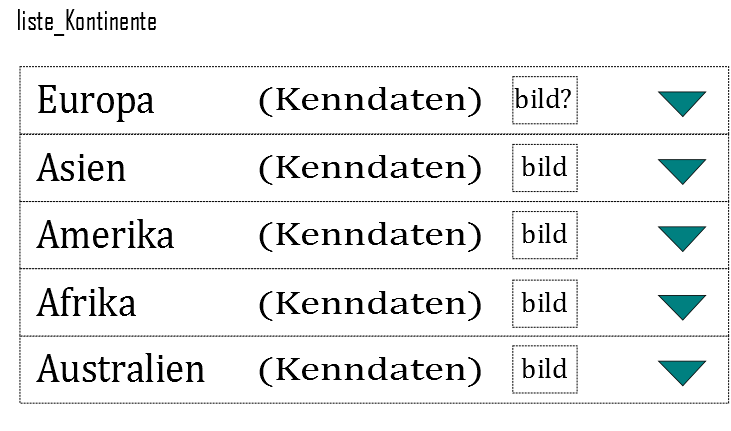
\includegraphics[width=0.4\textwidth]{images/Liste_Kontinente.PNG}}
			\hspace{1cm}
		 \subfigure[Bezeichnung der rechte Grafik]{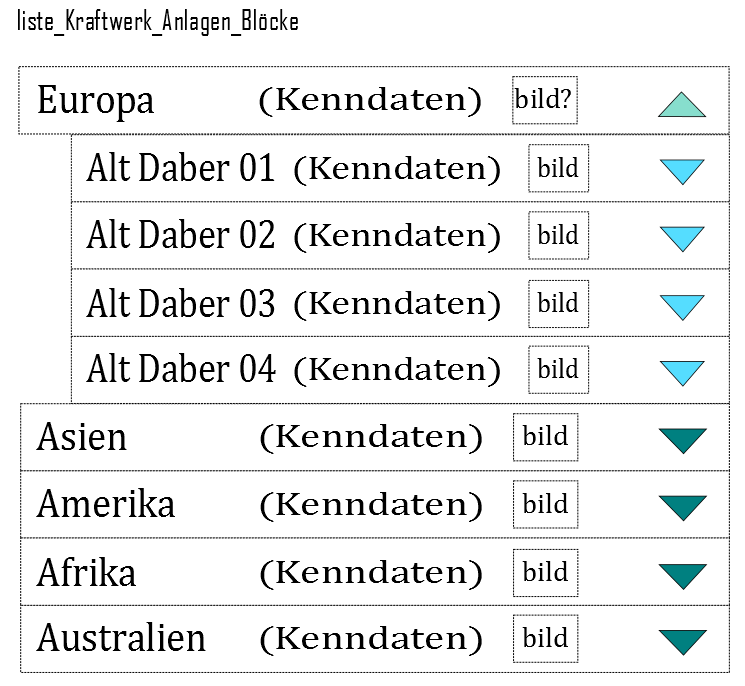
\includegraphics[width=0.4\textwidth]{images/Liste_Anlagenblocke.PNG}}
	\caption{Liste Anlagenbl�cke}
  \label{Anlagenblocke}
\end{figure}

\section{Nutzen von Bootstrap Frameworks, HTML, CSS f�r die Visualisierungen}

\Large{Mit Website-Tools, Sprachen, Frameworks habe ich erste Konzepte realisiert und die Elementen dargestellt}


% Key-Components: mit welchen Mitteln die Daten visualisieren = Bootstrap, JS, jQuery und andere\\


\section{Mittels FTP die Seite online stellen}

\Large{Kollegen haben einen Server erstellt, wo ich die Website ver�ffentlichen soll, damit die online verf�gbar ist}



\section{Mit SQL Database arbeiten und Meta-Datenbanken erstellen}

\Large{Verbinden von Daten aus SQL, Meta-Datenbank erstellt, welche die Allgemeine Infos und Daten zu Kraftwerk beinhaltet, Einen System erstellt und die Datenbank �ber SQL Sprache erstellt}



\section{Mit JS, jQuery, PHP dynamische Umsetzung und SQL Datenbanken verbinden}

\Large{Eine Dynamische Umsetzung erfolgt mittels PHP und andere.. es ist wichtig, dass die Seite dynamisch funktioniert, dass es automatisiert ist und wenn wir die SQL erweitern dann wird es automatisch im Website angezeigt}

% Key-Features: die Ajax Abfragen - aktualisieren von Daten, Daten aus der EBU, WR, BMS, Pool und evtl. noch weiteren visualisieren\\



\section{Mit Hilfe von Diagramm-Bibliotheken die Daten aus Datenbanken visualisieren}

\Large{Die Daten die im SQL liegen werden mittels Diagrammen visualisiert, es gibt mehrere Diagrammen-Bibliotheken, die man benutzen kann,  es war wichtig, dass die Open-source, mit SQL arbeiten kann - dynamisch, viele Optionen wie Export, mehrere Linien anzeigen, mehrere Typen von Charts, Datum-anzeigen}

% Charts-Plattform, welche Diagramm-Bibliothek benutzen wir? = meine Aufgabe war eine Auswahl von Charts machen, den besten finden und lernen damit die Daten visualisieren\\